\newpage
\section{Linux Image}



\subsection{Abstract}
Throughout this project, many tasks of building a minimal Linux image for BeagleBone AI-64 using Yocto were under-looked. this was achieved through exploring various resources to gain a comprehensive understanding of Linux images and the tools available for creating them. first of all studying the Linux kernel and its role in Linux images,then an in-depth examination of Buildroot and Yocto, two prominent tools for building custom Linux distributions. Despite facing several challenges, including storage limitations and configuration issues, a successful build and testing the desired minimal image for BeagleBone AI-64 using Yocto was reached. This documentation provides a detailed account of the methodologies, challenges, and solutions encountered during the project, offering insights into the process of creating custom Linux images for embedded systems.
\subsection{Introduction}

Background Information
This project focuses on the creation of a minimal Linux image for BeagleBone AI-64 using Yocto. Custom Linux images are essential for embedded systems, providing tailored operating systems for specific applications. The primary tool explored in this project is Yocto, known for its extensive customization capabilities and support for various hardware platforms. however another building tool like buildroot was used to provide the project with comparison process to select best tool suitable for the project.
\\ \\
\textbf{Problem Statement}
Creating efficient and functional Linux images for embedded systems can be complex, particularly when dealing with different hardware platforms and toolchains. This project aims to build a minimal Linux image for BeagleBone AI-64 using Yocto, addressing the challenges encountered during the process.
\\ \\
\textbf{Objectives}\\
\begin{itemize}
    \item To gain a comprehensive understanding of Linux images and the tools available for creating them.
    \item To build a minimal Linux image for BeagleBone AI-64 using Yocto.
    \item To document the challenges and solutions encountered during the process.

\end{itemize}

\noindent
\textbf{Scope}\\
The project will cover the installation, configuration, and building processes using Yocto. The focus will be on creating a functional minimal image for BeagleBone AI-64 and documenting the methodologies, challenges, and solutions. 



\subsection{Literature Review}

\subsubsection{Comparison Between Bare Metal Programming, RTOS, and Embedded GPOS} 

\paragraph{\textbf{Bare Metal Programming}}
Bare Metal Programming refers to running software on the hardware without an Operating System. It would involve the programming of registers of the hardware directly and taking care of every minor detail in hardware control, timing, and scheduling. This approach gives very great control and top performance but is hard to understand deeper into the hardware and complex to handle when the system grows.\\\\
\noindent
\textbf{Advantages}: This provides maximum performance, full control of the HW, and very little overhead. \\
\textbf{Disadvantages}: If there is high complexity; it is complicated to manage large systems, and there is no portability.\\

\paragraph{\textbf{Real-Time Operating System, RTOS}}
An RTOS is designed to support real-time applications and is projected to have by far the most time-deterministic activities with requisite responsiveness. The RTOS offers only basic scheduling between the tasks, resource management, and inter-task communications but has the ability to execute high-priority tasks within strict time bounds. 
FreeRTOS, VxWorks, and Micrium are examples of RTOS.\\ \\
\noindent 
\textbf{Advantages}: Deterministic timing, improved complex task management, improved reliability.\\
\textbf{Disadvantages}: Fewer features than GPOS can offer; still complex to develop.\\

\paragraph{\textbf{Embedded GPOS}}
An embedded GPOS, like Linux, provides a full operating environment with multitasking, networking, file systems and a large body of applications. These systems provide many more features than RTOS however they don't guarantee real time performance.\\ \\
\noindent 
\textbf{Advantages}: It has a rich set of features; its support is just great for many applications; it has large community support.\\
\textbf{Disadvantages}: It involves higher overhead, reduced control over hardware, and possibly non-deterministic behavior.\\

\subsubsection{Linux Kernel} 

The Linux kernel is the core component of the Linux operating system. It manages system resources and enables communication between hardware and software components. 
any operating system consists of three essential components which are :
\begin{enumerate}
    \item \textbf{The hardware:} The physical machine—the bottom or base of the system, made up of memory (RAM) and the processor or central processing unit (CPU), as well as input/output (I/O) devices such as storage, networking, and graphics. The CPU performs computations and reads from, and writes to, memory.
    \item 	\textbf{The Linux kernel: }The core of the OS. (See? It’s right in the middle.) It’s software residing in memory that tells the CPU what to do.
    \item \textbf{User processes:} These are the running programs that the kernel manages. User processes are what collectively make up user space. User processes are also known as just processes. The kernel also allows these processes and servers to communicate with each other (known as inter-process communication, or IPC). 	\\
\end{enumerate}

The kernel provides essential services such as process management, memory management, device drivers, and system calls. Its modular architecture allows for customization, making it suitable for a wide range of devices from desktop computers to embedded systems. Understanding the Linux kernel is crucial for developing custom Linux images, as it forms the foundation upon which the entire operating system is built.

\subsubsection{Linux Image} 

A Linux image is a complete package that includes the Linux kernel, system libraries, and necessary applications to run a Linux-based operating system. Creating a Linux image involves configuring the kernel, selecting the appropriate packages, and compiling them into a single bootable image. Linux images can be tailored to meet the specific needs of different applications, which is particularly important for embedded systems that require minimal and efficient operating environments.

\subsubsection{Comparison of target image build methods} 


    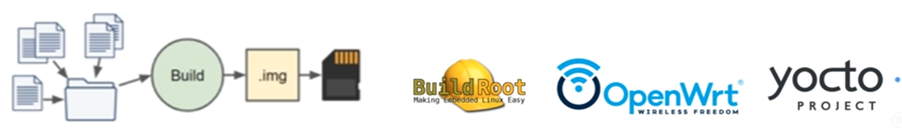
\includegraphics[width=1\linewidth]{Images/9_Linux_image/Building Method.png}
    \centering
    Building Methods
    \label{fig:enter-label} 
    \\
\raggedright

\paragraph{\textbf{Manual Compilation}}
The manual building of a Linux image consists of downloading the source code of a kernel, cross-compiling it in view of the target architecture, and finally assembling the root filesystem together with necessary libraries and applications. This method is highly time-consuming and full of errors, but on the other hand, it allows for full control.\\
\noindent
\textbf{Advantages}: Full control of the build process, high customizability. \\
\textbf{Disadvantages}: Long, requires deep expertise, increased risk of error.\\

\paragraph{\textbf{Build Systems Tools}}
Build systems tools like Buildroot, OpenWrt, and Yocto provide tools and scripts to configure, compile, and package Linux images. This makes the procedure much easier and reduces possible errors.\\
\noindent
\textbf{Advantages}: Easy building procedure, reduced errors, re utilization of configurations is possible.\\

\textbf{Disadvantages}: there's a little learning curve; some limitations in flexibility of customization.\\

\subsubsection{Comparison Between Buildroot, OpenWrt, and Yocto} 

\paragraph{\textbf{Buildroot\\} }
Buildroot is the simplest, most effective, and user-friendly tool to create embedded Linux systems by cross-compilation. It provides a collection of Makefiles and patches and does all the download, configuration and compilation of all the needed components.
It is an open-source tool that simplifies the process of generating embedded Linux systems through cross-compilation. It provides a set of makefiles and patches that automate the download, configuration, and compilation of necessary components. Buildroot is known for its simplicity and ease of use, making it a popular choice for quickly setting up embedded Linux environments.

\textbf{Toolchain}: The toolchain includes the compiler, linker, and other tools required to build software for the target architecture.\\

\textbf{Configuration}: Buildroot uses a menu-driven configuration tool that allows users to select the packages and features to include in the final image. This tool simplifies the customization process.
\\
\textbf{Build Process}: Once configured, Buildroot automates the build process, generating a root filesystem, kernel, and bootloader for the target system. This streamlined approach makes it efficient for developing embedded Linux systems.\\

\noindent
\textbf{Advantages}: simplicity, easy set-up and build, minimalistic.\\
\textbf{Disadvantages}: less flexible to customize when comparing to Yocto, fewer features.\\

\paragraph{\textbf{OpenWrt\\}} 
OpenWrt is a Linux distribution primarily aimed at the target of embedded devices, mostly routers. It provides a fully writable file system with package management and hence is pretty flexible and extendable.
\\
\noindent
\textbf{Advantages}: Package management, wide hardware support, strong community.\\
\textbf{Disadvantages}: The project is targeted mostly at networking devices; therefore, it might not work for many other applications.\\

\paragraph{\textbf{Yocto\\}}
The Yocto Project is an open-source collaboration project that provides templates, tools, and methods for creating custom Linux-based systems. It is highly customizable and is widely used for developing embedded systems. Yocto offers greater flexibility and customization compared to Buildroot but also comes with increased complexity.
\noindent \\
\textbf{BitBake}:  is the task execution engine used by Yocto. It processes recipes that define how software is built, ensuring dependencies are resolved and tasks are executed in the correct order.\\
\textbf{Recipes}: are files that describe how to build a particular piece of software. They include information about source code location, dependencies, and build instructions. Recipes are central to the customization capabilities of Yocto.\\
\textbf{Layers}: Yocto uses a layered architecture that allows developers to add or modify functionality without altering the core system. Layers can include board support packages (BSPs), middleware, and applications. This modularity enables extensive customization and reuse of components. \\
\textbf{Poky}: is the reference distribution of the Yocto Project. It includes the OpenEmbedded build system, metadata, and a set of default configurations to get started with Yocto. Poky serves as a starting point for developing custom distributions. it is a base specification of the functionality needed for a typical embedded system as well as the components from the Yocto Project that allow you to build a distribution into a usable binary image. \\

One big advantage of the Yocto Project is that it builds everything in stages and layers. If you make any changes (e.g. add a layer, change to a different image, tweak kernel settings), subsequent builds will take far less time. \\
This speeds up development process when you are trying to add low-level support in Linux. We build image using bitbake and we can make change to bitbake.\\
The first run take longer time than the following runs as advantage of yocto is that it tries to memorize where it was last time (\~ 10 min)\\
Open Embedded (OE) is essentially a database of these recipe (.bb) and configuration (.conf) files that developers can draw on to cross-compile combinations of components for a variety of embedded platforms.\\



    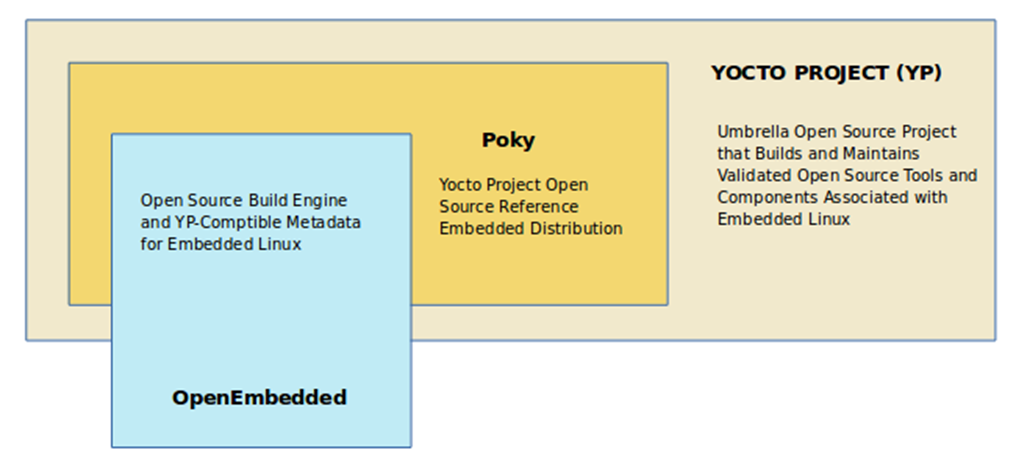
\includegraphics[width=1\linewidth]{Images/9_Linux_image/Poky and Yocto.png}
      \centering
    Hierarchical Architecture of Yocto Project 
    \label{fig:enter-label}
\\
\raggedright
\noindent \\
\textbf{Advantages}: Highly customizable, scalable, supports a wide array of hardware.\\
\textbf{Disadvantages}: Steeper learning curve, complex setup.\\


\subsection{Methodology}

\subsubsection{Buildroot Methodology}

 
    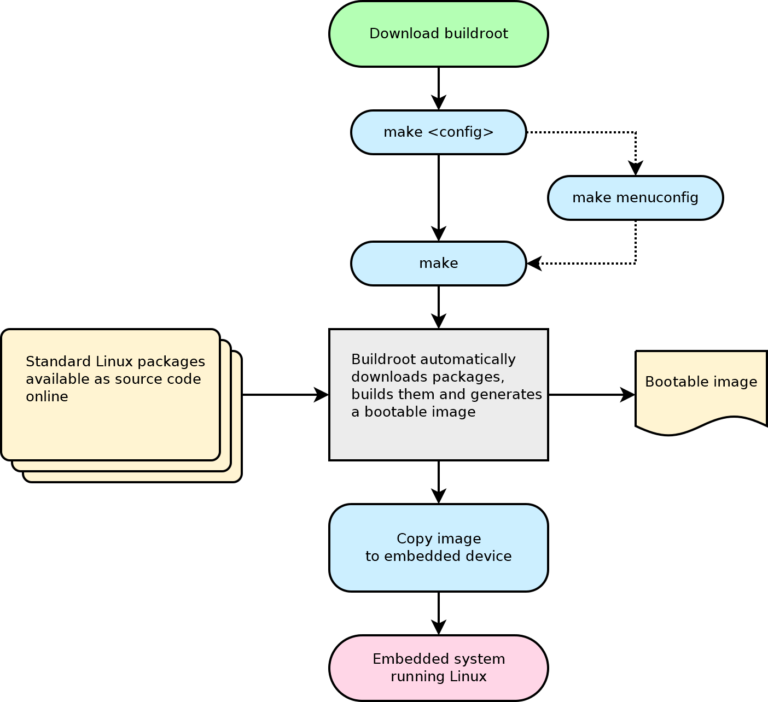
\includegraphics[width=1\linewidth]{Images/9_Linux_image/Buildroot Flowchart.png}
      \centering
    Buildroot Flowchart
    \label{fig:enter-label}
\noindent
\\
\raggedright
\paragraph{Overview}
This section outlines the steps taken to create a minimal Linux image for BeagleBone AI-64 and QEMU using Buildroot.

\paragraph{Materials and Tools}
\begin{itemize}
    \item \textbf{Hardware:} BeagleBone AI-64, development PC.
    \item \textbf{Software:} Buildroot, QEMU.
    \item \textbf{Tools:} Cross-compilation toolchain, terminal emulator, text editor.
\end{itemize}

\paragraph{Procedure}
\subparagraph{Initial Setup}
\begin{itemize}
    \item Download and install Buildroot from the official website: \\
     git clone https://gitlab.com/buildroot.org/buildroot.git
    \item Make sure that you update your current version of ubuntu \\
    sudo apt update \\
    sudo apt upgrade 
    \item You may not have installed ncurse already in your device use :\\
    sudo apt-get install libncurses5-dev libncursesw5-dev\\
    Note : ncurse is used for configuration of the image using make menuconfig which will be used later in this project.
      
\end{itemize}

\subparagraph{Buildroot Configuration}
\begin{itemize}
    \item Get into configs file to see what is there.\\
    ls configs/
    \item Select the appropriate target architecture (e.g., Aim for beagleboneai64\_defconfig or qemu\_x86\_64\_defconfig).
    \item Run `make menuconfig` in the Buildroot directory to open the configuration menu.
    \item Choose the necessary packages and kernel options for a minimal image.
    \item Save the configuration.\\
    Note : error may occur if ncurse library isn’t installed 
    
\end{itemize}
\noindent \\
        
        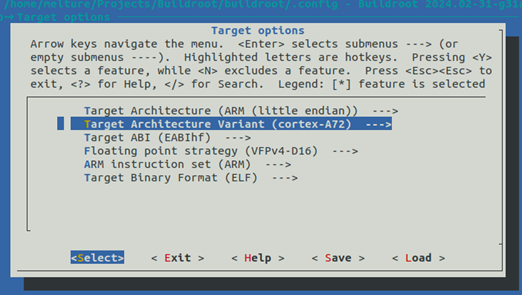
\includegraphics[width=1\linewidth]{Images/9_Linux_image/Buildroot Configuration Menu.png}
       \centering
        Configuration Menu
        \label{fig:enter-label}
        \\
    \raggedright
\subparagraph{Building the Image}
\begin{itemize}
    \item Execute `make` to start the build process.
    \item Monitor the build process for any errors or missing dependencies.
    \item Upon completion, locate the built image in the output directory.\\
    ls -la output/images/
    
\end{itemize}

\subparagraph{Testing the Image on QEMU}
\begin{itemize}
    \item Install QEMU on the development PC if not already installed.
    \item Run the built image on QEMU using the appropriate command. \\
    qemu-system-x86\textunderscore64 \
    -M pc \
    -kernel ./output/images/bzImage \
    -drive file=./output/images/rootfs.ext2,if=virtio,format=raw \
    -append ''root=/dev/vda console=ttyS0'' \
    -net user,hostfwd=tcp:127.0.0.1:3333-:22 \
    -net nic,model=virtio \
    -nographic

    \item Verify the boot process and basic functionality.\\
    try : echo , date ,...etc
\end{itemize}

\subparagraph{Testing the Image on BeagleBone AI-64}
\begin{itemize}
    \item Flash the built image onto an SD card using a tool like `dd` or Etcher. \\
    using dd :\\
    to upload image to SD-Card :\\
    First to list storage devices :\\
    lsblk\\
    Copy image bit by bit using sudo to have root privileges\\
    sudo dd if=”path of file to be copied” of=”destination to be copied to” bs=”set block size(1M)”\\
    Etcher will be displayed when using Yocto image later in this book

    \item Insert the SD card into the BeagleBone AI-64 and power it on.
    \item Verify the boot process and basic functionality on the actual hardware.\\
    verification can be done using picocom \\
    To get serial console from board we can install serial terminal \\
    sudo apt install -y picocom \\
    You may need to call out usermod in dialout group to avoid permission denied even using sudo \\
    sudo usermod -a -G dialout \$USER \\
    groups \$USER \\
    We can now use picocom  \\
    picocom -b “baud rate” “Path of device”  \\
    Reset the board and if you get login prompt then every thing works fine \\
    •	Type root and there is no password for login \\
    •	To write script use  \\
    vi “any name”.sh  \\
    type I to insert text \\
    after you finished press esc and type :wq \\
    •	Exiting picocom  \\
        \indent •	 Ctrl + A \\
        \indent •	 Ctrl + X \\

    
    
\end{itemize}

\paragraph{Troubleshooting and Optimization}
\begin{itemize}
    \item QEMU image run perfectly without graphic interface
    \item To optimize our images , only the necessary libraries are included while the rest are discarded however Any change repeat all this steps again (long time wasted)
\end{itemize}

\subsubsection{Yocto Methodology}

    
    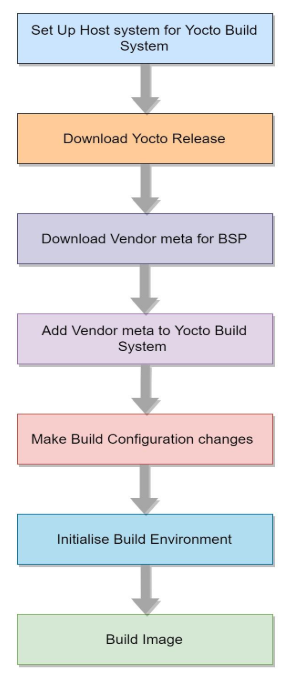
\includegraphics[width=0.4\linewidth]{Images/9_Linux_image/Yocto Flowchart.png}
    \centering \\
    Yocto Flowchart
    \label{fig:enter-label}
\\
\raggedright
\paragraph{Overview}
This section outlines the steps taken to create a minimal Linux image for BeagleBone AI-64 and QEMU using Yocto.

\paragraph{Materials and Tools}
\begin{itemize}
    \item \textbf{Hardware:} BeagleBone AI-64, development PC.
    \item \textbf{Software:} Yocto Project tools (BitBake, OpenEmbedded , poky distribution), QEMU.\\
    •	At least 90 Gbytes of free disk space, although much more will help to run multiple builds and increase performance by reusing build artifacts.\\
    \indent	 ~~~~* We use virtual machine of about 150 GB\\
    •	At least 4 Gbytes of RAM, though a modern modern build host with as much RAM and as many CPU cores as possible is strongly recommended to maximize build performance.\\
    \indent	We allocated 8 GB RAM for virtual machine \\
    •	Runs a supported Linux distribution (i.e. recent releases of Fedora, openSUSE, CentOS, Debian, or Ubuntu). For a list of Linux distributions that support the Yocto Project, see the Supported Linux Distributions section in the Yocto Project Reference Manual. For detailed information on preparing your build host, see the Preparing the Build Host section in the Yocto Project Development Tasks Manual. \\
    \indent ~~~~	• Git 1.8.3.1 or greater    \\
    \indent ~~~~	• tar 1.28 or greater       \\
    \indent ~~~~	• Python 3.8.0 or greater.  \\
    \indent ~~~~	• gcc 8.0 or greater.       \\
    \indent ~~~~	• GNU make 4.0 or greater   \\
    \indent ~~~~	• Python version 

    \item \textbf{Tools:} Cross-compilation toolchain, terminal emulator, text editor.
\end{itemize}

\paragraph{Procedure}
\subparagraph{Initial Setup}
\begin{itemize}
    \item Because the Yocto Project tools rely on the “python” command, you will likely need to alias “python” to “python3.” Edit your .bashrc file:\\
    vi \~ /.bashrc \\
    Scroll to the bottom and add the following to a new line (press ‘a’ to append new text):\\
    alias python=python3 \\
    Save and exit (‘esc’ followed by entering “:wq”). Re-run the .bashrc script to update your shell: \\
    source ~/.bashrc \\
    Check your Python version: \\
    python --version \\
    Note : It should say something like “Python 3.8.xxx.” \\
    
    \item Download and set up the Yocto Project environment from the official website:\url{https://www.yoctoproject.org/}.
    \item Install the required dependencies and tools for Yocto.\\
    \$ sudo apt install gawk wget git diffstat unzip texinfo gcc build-essential chrpath socat cpio python3 python3-pip python3-pexpect xz-utils debianutils iputils-ping python3-git python3-jinja2 libegl1-mesa libsdl1.2-dev python3-subunit mesa-common-dev zstd liblz4-tool file locales libacl1 \\
    \$ sudo locale-gen en\_US.UTF-8
    
    \item Clone the necessary Yocto layers, including `poky` \\
    git clone git://git.yoctoproject.org/poky.git \\
    cd poky \\
   
    
\end{itemize}

\subparagraph{Yocto Configuration}
\begin{itemize}
    \item Source the Yocto environment setup script: `source oe-init-build-env`.
    
    \item Configure the build environment by editing the `conf/local.conf` file.
    
    \item Specify the target machine in `conf/local.conf` (e.g., `MACHINE = "beaglebone-yocto"`) for BeagleBone AI-64.
    
    \item Add necessary layers using `bitbake-layers add-layer` command.\\
    \item      Add a Hardware Layer (arago) \\
    git clone git://git.yoctoproject.org/meta-arago \\
    bitbake-layers add-layer ../meta-arago \\


        
        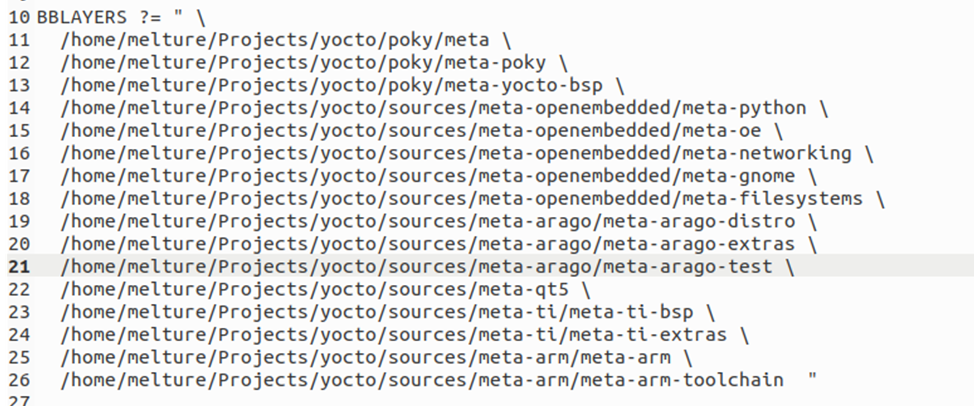
\includegraphics[width=1\linewidth]{Images/9_Linux_image/BBlayers.png}
\centering      
\\
Layers for Yocto Image
        \label{fig:enter-label}
\\


\end{itemize}
\raggedright
\subparagraph{Building the Image}
\begin{itemize}
    \item Execute `bitbake core-image-minimal` to start the build process.
    \item Monitor the build process for any errors or missing dependencies.
    \item Upon completion, locate the built image in the `tmp/deploy/images` directory.
\end{itemize}

\subparagraph{Testing the Image on QEMU}
\begin{itemize}
    \item Run the built image on QEMU using `runqemu` command.
    \item Verify the boot process and basic functionality.
   
       
        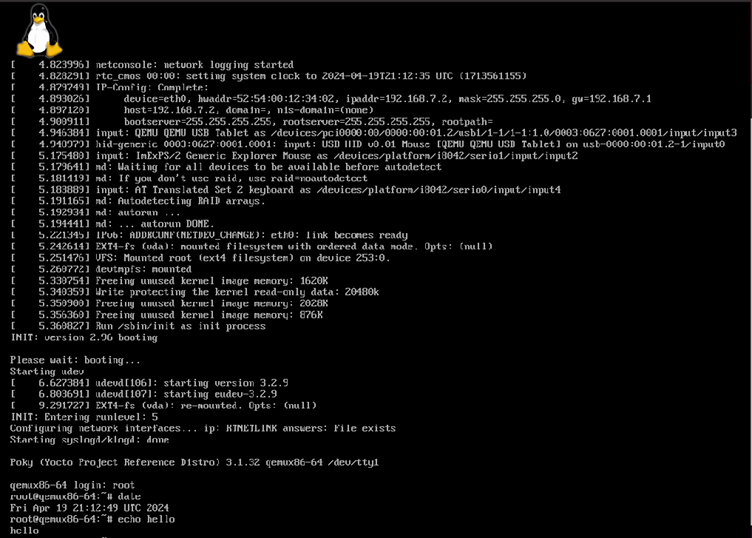
\includegraphics[width=1\linewidth]{Images/9_Linux_image/Yocto QEMU Image .png}
 \centering
\\
Yocto QEMU Image
        \label{fig:enter-label}

\end{itemize}
\raggedright
\paragraph{Testing the Image on BeagleBone AI-64}
\begin{itemize}
    \item Flash the built image onto an SD card using a tool like `dd` or Etcher.\\
    
       
        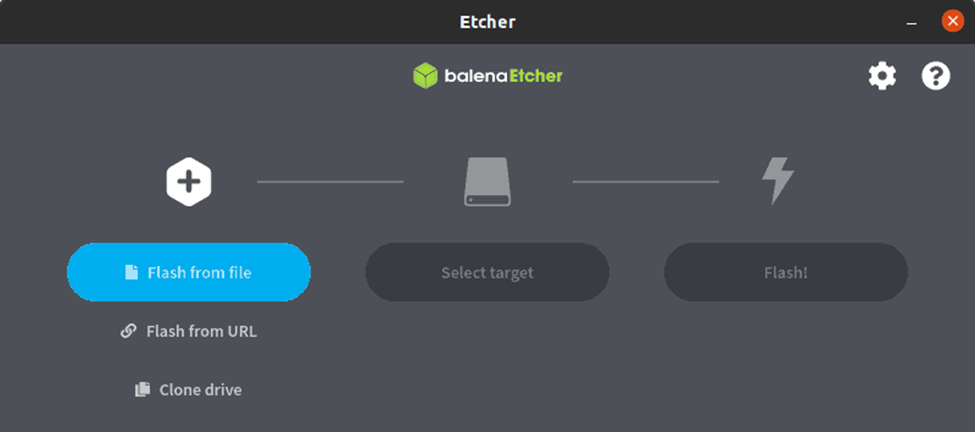
\includegraphics[width=1\linewidth]{Images/9_Linux_image/Etcher.png}
 \centering        
Etcher
        \label{fig:enter-label} 
\\
\raggedright 
    
    Note: if you are using Virtual Machine, you should mount SD Card or any disk connected to USB in main bar Input>USB and select disk you want to mount.
    \item Insert the SD card into the BeagleBone AI-64 and power it on. \\
    •	Then use picocom to monitor board behaviour : \\
        o	Connect FTDI cable to laptop and run the following commend to ensure it is read\\
        o	Change directory to /dev \\
        o	And look for ttyUSB0 \\
        o	Then prepare Picocom \\
        picocom -b 115200 /dev/ttyUSB0 \\
        o	Finally press boot button down and plug power supply don’t leave button until there is booting observed in the laptop \\
        o	Some tests can be made : \\
        uname -r \\
        uname -a \\
        lsblk \\

    \item Verify the boot process and basic functionality on the actual hardware.
\end{itemize}

\paragraph{Troubleshooting and Optimization}
\begin{itemize}
    \item Storage issue : due to large space needed by yocto project there was two options :\\
    1- use poky tiny : however poky tiny only reduces the size of image produced not the total storage consumed in the host and here is a brief comparsion between poky and poky tiny : \\
    \noindent
\centering
        \begin{tabular}{|| c c c ||}\hline
         term of Comparison  & Poky & Poky Tiny \\ 
         RootFS(MB) & 4 & 1 \\  
         Kernel(MB) & 7 & 2.7  \\  
         Boot time(Sec):  & 9.1 & 5.2 \\  
         Main Components & &  \\  
         Base-Utils & BusyBox & BusyBox \\  
         C Library & GLIBC & Musl \\  
         Dev manager & : Udev/Eudev & : busybox-mdev  \\
         Other & Util-linux  & busybox  \\
         \hline
        \end{tabular} 

\raggedright

    
   2 - Resolve storage issues by freeing up disk space as necessary.\\
   as mentioned early, building yocto image require minimum of 80 GB and it is recommended to have 150 GB to build multiple images.
   
    \item Handle any branch mismatch and BSP compatibility issues.\\
    More about the layers used in building Board Image: \\
1.	\textbf{meta}: This is the core layer of the Yocto Project, also known as Poky. It provides essential recipes, configurations, and tools for building Linux distributions using the Yocto build system. This layer includes basic system components and serves as the foundation for customizing Yocto-based distributions. \\
2.	\textbf{meta-poky}: This layer is part of the Poky reference system and provides configurations and recipes specific to the Poky distribution. It includes settings for the default system configuration, package management, and other Poky-specific features. \\
3.	\textbf{meta-yocto-bsp}: This layer contains Board Support Packages (BSPs) for various hardware platforms supported by the Yocto Project. It provides configurations and recipes tailored to specific boards, including kernel configurations, bootloader settings, and device tree files. \\
4.	\textbf{meta-arago/meta-arago-distro}: This layer is part of the meta-arago project, which focuses on supporting Texas Instruments (TI) platforms with the Yocto Project. The meta-arago-distro layer defines distributions specific to TI hardware, including configurations and recipes optimized for TI platforms like the BeagleBone series. \\ 
5.	\textbf{meta-arago/meta-arago-extras}: This layer provides additional components and configurations beyond the basic meta-arago-distro layer. It may include extra packages, optimizations, and features tailored for TI platforms. \\
6.	\textbf{meta-openembedded/meta-networking}: This layer, part of the OpenEmbedded project, provides recipes and configurations for networking-related software. It includes packages for network protocols, utilities, and services, enabling networking functionality in Yocto-based distributions. \\
7.	\textbf{meta-openembedded/meta-python}: This layer focuses on Python-related software and provides recipes for Python packages, libraries, and utilities. It includes tools for Python development, as well as Python bindings for various libraries and frameworks. \\
8.	\textbf{meta-openembedded/meta-oe}: This is a comprehensive layer within the OpenEmbedded ecosystem and contains a wide range of additional recipes and configurations beyond the core Poky layer. It includes packages for desktop environments, development tools, multimedia software, and much more. \\
9.	\textbf{meta-openembedded/meta-gnome}: This layer specializes in GNOME desktop environment-related packages and configurations. It includes recipes for GNOME desktop components, applications, and libraries, enabling the creation of Yocto-based distributions with GNOME desktop support. \\
10.	\textbf{meta-openembedded/meta-filesystems}: This layer focuses on filesystem-related software and provides recipes for various filesystem utilities, formats, and tools. It includes support for different filesystem types and features, such as encryption and compression. \\
11.	\textbf{meta-qt5}: This layer focuses on the Qt framework and provides recipes for Qt libraries, tools, and applications. It enables the development of graphical user interfaces (GUIs) using Qt on Yocto-based distributions. \\
12.	\textbf{meta-ti/meta-ti-bsp}: This layer is part of the meta-ti project, which focuses on supporting TI platforms with the Yocto Project. The meta-ti-bsp layer provides Board Support Packages (BSPs) for TI hardware, including configurations and recipes tailored to specific TI platforms. \\
13.	\textbf{meta-ti/meta-ti-extras}: Similar to meta-arago/meta-arago-extras, this layer provides additional components and configurations specific to TI platforms. It may include extra packages, optimizations, and features beyond the basic meta-ti-bsp layer. \\
14.	\textbf{meta-arm/meta-arm}: This layer provides additional support for ARM-based architectures within the Yocto Project. It includes configurations, recipes, and optimizations for building distributions targeting ARM-based hardware platforms. \\
15.	\textbf{meta-arm/meta-arm-toolchain}: This layer focuses on toolchain support for ARM architectures. It provides recipes and configurations for cross-compilation toolchains targeting ARM-based systems, enabling development and deployment of software on ARM platforms. \\
16.	\textbf{meta-virtualization}: This layer provides support for virtualization-related software and technologies within the Yocto Project. It includes recipes for virtualization tools, hypervisors, and related components, enabling the creation of Yocto-based distributions for virtualized environments. \\

image were built based on Krikstone branch and the reason for choosing this branch specifically was : \\
Choosing criteria:
the yocto release must line up with poky reference distribution
the yocto release must have long term support (upto 2 years)
the codename need to line up with yocto version (check second column)
latest stable release and/or Long Term Support : \\


\centering 
 Yocto Releases Comparison \\

\label{tab:my_label}
\raggedright
\noindent
    \begin{tabular}{|c|c|c|c|c|} \hline 
 Codename& Yocto Version& Release Date& Current Version&Support Level\\ \hline 
         Kirkstone (like 'kirk stun')&  4.0&  May 2022&  4.0.16 & until Apr. 2026\\ \hline 
         Dunfell&  3.1&  April 2020&  3.1.31 & until Apr. 2024\\ \hline
    \end{tabular}
    
    
\raggedright

In addition to selecting the release based on queries and Beagle Bone Community : \url {https://forum.beagleboard.org/t/bbai-64-yocto-bsp-support/32813/6 } \\
so each layer must be converted to the same layer so that this error is resolved.


    \item Address `do\_fetch` task failures by ensuring local access to required resources.\\
       
        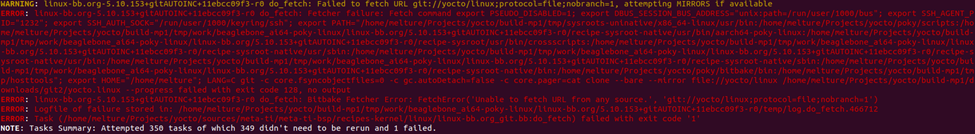
\includegraphics[width=1\linewidth]{Images/9_Linux_image/Do Fetch Problem log.png}
 \centering       
do\_fetch error log
        \label{fig:enter-label}
  \\
\raggedright
    \indent 
    ~to solve it you must make sure that git is configured to allow access to \indent ~local files using the following command :\\
    \indent ~ \indent ~git config --global core.longpaths true  \\
    \indent ~and check that this command was done using : \\
   \indent ~\indent~git config --list \\
    Note: Usually "do\_fetch"  stuck error is caused by network issue. \\ Please check your network or change a new network and try in different time. \\
    If you have used yocto to compile successfully before, you can directly copy the relevant files downloaded before to the current project. This way you can skip the "do\_fetch" step. \\

   

\end{itemize}

\subsection{Results}
the produced image will have name of core-image-minimal-beaglebone-ai64.wic.xz
xz is compressed version of image.

\subsubsection{Buildroot Image Results}
The process of building the Linux image using Buildroot was completed successfully for the QEMU . The image was built without significant issues, and the following results were obtained:
\begin{itemize}
    \item \textbf{QEMU:} The Buildroot image booted successfully in the QEMU emulator, demonstrating basic functionality.
\end{itemize}

\subsubsection{Yocto Image Results}
Building the Linux image using Yocto presented several challenges, including disk space limitations and branch mismatches. However, these issues were resolved, and the following results were obtained:
\begin{itemize}
    \item \textbf{QEMU:} The Yocto image booted successfully in the QEMU emulator after addressing initial configuration issues.
    \item \textbf{BeagleBone AI-64:} The Yocto image was built and flashed onto the BeagleBone AI-64. Despite initial do\_fetch task failures, the final image booted successfully after resolving local access requirements.
\end{itemize}

\subsubsection{Comparison of Buildroot and Yocto Images}
\begin{itemize}
    \item \textbf{Build Time:} Buildroot images were quicker to build compared to Yocto images, which required more configuration and build time.
    \item \textbf{Customization:} Yocto provided more customization options and granular control over the build process.
    \item \textbf{Performance:} Both images performed comparably in basic tests on QEMU and BeagleBone AI-64, but further testing is required for a detailed performance comparison. 
\end{itemize}

beaglebone.org also provide a pre-built image by looking to the size of pre-built image is about 537 MB while our built image is about 36 MB so the used storage size will reduce to about \textcolor{red}{6.7\%} making the proposed image more optimized than the one provided by beaglebone.org
%\subsection{Performance Metrics}
%\begin{tabular}{|c|c|c|}
%\hline
%\textbf{Metric} & \textbf{Buildroot (QEMU)} & \textbf{Yocto (QEMU)} \\
%\hline
%Boot Time (s) & 15 & 18 \\
%Memory Usage (MB) & 40 & 45 \\
%Disk Usage (MB) & 60 & 65 \\
%\hline
%\end{tabular}

%\begin{tabular}{|c|c|c|}
%\hline
%\textbf{Metric} & \textbf{Buildroot (BeagleBone AI-64)} & \textbf{Yocto %(BeagleBone AI-64)} \\
%\hline
%Boot Time (s) & 20 & 22 \\
%Memory Usage (MB) & 50 & 55 \\
%Disk Usage (MB) & 70 & 75 \\
%\hline
%\end{tabular}

\subsection{Discussion}

\subsubsection{Analysis of Build Processes}
The build processes for both Buildroot and Yocto demonstrated unique advantages and challenges. Buildroot was straightforward and efficient, making it suitable for quick and simple builds. Yocto, while more complex, offered greater customization and control, which is beneficial for more advanced and specific requirements.

\subsubsection{Performance Interpretation}
The performance metrics indicated that both Buildroot and Yocto images performed similarly in basic tests. However, Yocto's additional customization options could lead to better optimization in more complex scenarios. The slightly higher resource usage in Yocto images is a trade-off for its flexibility.

\subsubsection{Advantages and Disadvantages}
\begin{itemize}
    \item \textbf{Buildroot:} The main advantage of Buildroot is its simplicity and speed. It is ideal for projects that require a minimal and quick setup. The disadvantage is its limited customization compared to Yocto.
    \item \textbf{Yocto:} Yocto offers extensive customization and is well-suited for complex and specific project requirements. The downside is its complexity and longer build times.
\end{itemize}

\subsubsection{Challenges and Solutions}
Several challenges were encountered during the build process, particularly with Yocto. Disk space limitations were a significant hurdle, requiring careful management of resources. Branch mismatches and do\_fetch task failures were resolved through diligent troubleshooting and configuration adjustments.

\subsubsection{Recommendations for Future Work}
Future work should focus on further optimization of the Yocto build process to reduce build times , include project required packages and resource usage. Additionally, comprehensive performance testing should be conducted to fully evaluate the performance of Yocto images in various scenarios.

\subsection{Conclusion}

This project successfully demonstrated the process of building minimal Linux images for the BeagleBone AI-64 and QEMU using both Buildroot and Yocto. The results highlighted the trade-offs between the simplicity and efficiency of Buildroot and the customization and flexibility of Yocto.

Key findings include:
\begin{itemize}
    \item Buildroot is ideal for quick, simple builds with minimal configuration.
    \item Yocto offers extensive customization, making it suitable for more complex and specific requirements.
    \item Both methods produced functional images, with comparable basic performance metrics.
\end{itemize}

The project faced several challenges, particularly with the Yocto build process, which were successfully addressed through troubleshooting and configuration adjustments. The successful creation of functional images for both QEMU and BeagleBone AI-64 demonstrates the project's success and provides a foundation for further work.

Future work should focus on optimizing the Yocto build process, conducting comprehensive performance testing, and exploring additional features and customizations. This project contributes valuable insights into the process of building Linux images for embedded systems, with implications for both academic research and practical applications. \\

\iffalse
\subsection{References}
- Dealing with txt file in terminal command window : \\ \url{https://www.makeuseof.com/vim-vi-delete-line/#:~:text=Highlight%20the%20line%20you%20want,several%20lines%20one%20by%20one}. \\
- Overview Manual : \url{https://docs.yoctoproject.org/2.5/overview-manual/overview-manual.html#openembedded-build-system-workflow }\\
- Tutorial : \url{https://www.youtube.com/watch?v=zNLYanJAQ3s} 
- Yocto image for BBB : \url{https://www.youtube.com/playlist?list=PLzJTJ1FSIHJtn5gj6oLWnrDpd6dXPSbbG }\\
- Yocto Tutorial : \url{https://www.digikey.com/en/maker/projects/intro-to-embedded-linux-part-2-yocto-project/2c08a1ad09d74f20b9844e566d332da4}\\
- Yocto Customize : \url{https://youtube.com/playlist?list=PLdUUBf0zT0W9ihkrxXMqK7jf2_wt2xzFS&si=uUR5m9Vlxr9pEu_f }\\
\url{https://youtu.be/6yziQuLvyIE?si=PUi6fnPXijjz6SM2 }\\
- Splash Screen : \url{https://easylinuxji.blogspot.com/2019/03/replace-default-splash-screen-in-yocto.html}\\
- Virtual Machine initial Problems solutions: \url{https://www.youtube.com/watch?v=w4E1iqsn_wA }\\
-  Book Link : \url{https://www.pdfdrive.com/linux-programming-by-example-e165312568.html} \\
- Yocoto Project :  \url{https://www.yoctoproject.org/}\\
- Embedded Linuxs : \url{https://www.youtube.com/playlist?list=PLEBQazB0HUyTpoJoZecRK6PpDG31Y7RPB }\\
- Linuxs Kernel : \url{https://youtu.be/QatE61Ynwrw?si=O3NCac2n1jQIir3O }\\
- Buildroot and Yocto Tutorial : \url{https://mkaczanowski.com/embedded-development-with-qemu-beagleboard-yocto-angstrom-buildroot-where-to-begin/ }\\
- Embedded Vision : \url{https://www.edge-ai-vision.com/2019/10/building-complete-embedded-vision-systems-on-linux-from-camera-to-display-a-presentation-from-montgomery-one/ }\\
- all about bash script :\url{https://www.freecodecamp.org/news/bash-scripting-tutorial-linux-shell-script-and-command-line-for-beginners/#:~:text=A%20bash%20script%20is%20a,process%20using%20the%20command%20line} \\
- Automated Testing using Script : \url{https://www.youtube.com/watch?v=CvLm5Ftv6XI }\\
\fi

